  
 
  
  
\begin{frame}\frametitle{Factors flow graph} 
  
  
\begin{center} 
  
  
\begin{figure} 
  
  
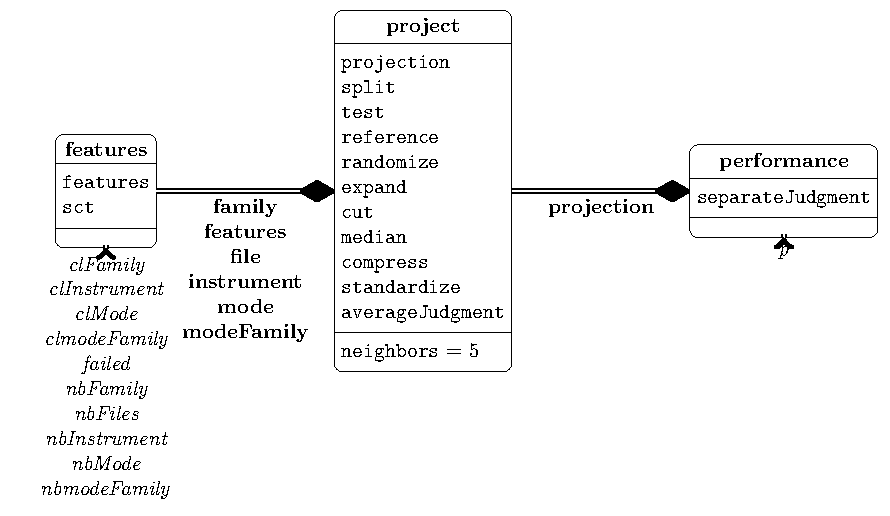
\includegraphics[width=\textwidth,height=0.8\textheight,keepaspectratio]{../figures/factors.pdf} 
  
  
\label{factorFlowGraph} 
  
  
\end{figure} 
  
  
\end{center} 
  
  
\end{frame} 
  
\begin{frame}\frametitle{features: tfscat, sct: 1000, split: none, reference: judgments, randomize: 0, median: 1, compress: 1, standardize: 1} 
  
\begin{table} 
\begin{center} 
\ 
 \setlength{\tabcolsep}{.16667em} 
\begin{tabular}{c} 
p (\%) \\ 
\hline 
\end{tabular} 
\end{center} 
\label{fetfSc1000SpnoRejuRa0Me1Co1St1} 
\end{table} 
 
\end{frame}  
